\chapter{Implementation, Integration and Testing}
\label{ch:implementation-integration-and-testing}%

\section{Overview and Implementation Plan}
\label{sec:overview-and-implementation-plan}%

\par In this chapter, we will discuss the implementation of the S\&C Web Application, the integration and the test
strategy that will be used to ensure the quality of the software. In general, the methodology used to implement the
S\&C Web Application is the Bottom-Up approach, which is a software development approach that starts by implementing
the lower-level modules first, and then integrating them to create higher-level modules.

\par By using this approach, we can ensure that the lower-level modules are working correctly before integrating them into
higher-level modules. Each module will require a Driver to test the module. The Driver will simulate the behavior of
the higher-level module and will call the lower-level module to test its functionality by making calls of the interfaces
given by the lower-level module.
The Bottom-Up strategy grants a step by step integration of the modules and ensures that the software is working correctly
thanks to the testing of each module, that will make easier to identify and fix the bugs of the different modules before
integrating them into more complex ones. This strategy also allows the development team to work on different modules
simultaneously, which can speed up the development process.


\section{Features Identifications}
\label{sec:features-identifications}%

\par The S\&C Web Application is a complex software that has different features that are going to be used by the different
users. The features are divided into three main categories: the CO Features, the ST Features, and the UN Features. Each
category has different features that are going to be used by the different users. The features are identified as follows:

\par \textbf{CO Features}: This set of features is used by the COs to manage their profile, the internships
advertisement that they will create, their editing, the creation of the questionnaires, the management of the applicants
lists and the management of the internships.

\begin{itemize}
    \item \textbf{[CO.1] Profile Management}: This feature allows the COs to manage their profile, by changing their
          CO's information, such as the description provided and the CO's logo.
    \item \textbf{[CO.2] COs' Questionnaires Management}: This feature allows the COs to create, edit and delete the
          questionnaires that they will send to the applicants that have applied to their internships.
    \item \textbf{[CO.3] Internship Advertisement Management}: This feature allows the COs to create, edit and delete
          the internships advertisements.
    \item \textbf{[CO.4] Internship Progress Management}: This feature allows the COs to see the applicants that have
          applied to their internships, to visualize the applicants' information, to select the applicants that they want to
          send the interview questionnaires and to set the deadlines for the applicants to answer the questionnaires.
    \item \textbf{[CO.5] System's Questionnaires Answering}: This feature allows the COs to answer the feedback
          questionnaires that the system will send to them after the internships have ended.
\end{itemize}

\par \textbf{ST Features}: This set of features is used by the STs to manage their profile, to apply to the 
internships and to answer the questionnaires sent by the COs.

\begin{itemize}
    \item \textbf{[ST.1] Profile Management}: This feature allows the STs to manage their profile, by changing their
          ST's information, and to load their CV.
    \item \textbf{[ST.2] Internship Advertisement Application}: This feature allows the STs to apply to the internships
          advertisements that they are interested in.
    \item \textbf{[ST.3] COs' Questionnaires Answering}: This feature allows the STs to answer the questionnaires sent by
          the COs and to see the deadlines for the questionnaires.
    \item \textbf{[ST.4] Internship Progression}: This feature allows the STs to see the status of the internships
          advertisement that they have applied to.
    \item \textbf{[ST.5] System's Questionnaires Answering}: This feature allows the STs to answer the feedback
          questionnaires that the system will send to them after the internships have ended.
\end{itemize}

\par \textbf{UN Features}: This set of features is used by the UN's staff to visualize the information of the
internships to which it's students are involved, the contracts that the UN has with S\&C, and the ability to block the
COs that are not following the terms of the application.

\begin{itemize}
    \item \textbf{[UN.1] Internships Information Visualization}: This feature allows the UN's staff to see the
          information and the status of the internships to which it's students are involved.
    \item \textbf{[UN.2] Contracts Visualization}: This feature allows the UN's staff to see the contracts that the UN
          has with S\&C.
    \item \textbf{[UN.3] COs' Blocking}: This feature allows the UN's staff to block the COs.
\end{itemize}


\par This feature identification is useful to identify what the different users can do in the Web Application. 
Now it's going to be discussed how the different features are going to be implemented based on the architecture given in
chapter \ref{ch:architectural-design}:

\par \textbf{[F1] Login Features}: 

\begin{itemize}
    \item \textbf{[F1.1] Login by SSOs}: This feature allows the STs and the UN's staff to login into the Web Application
          using their SSOs.
    \item \textbf{[F1.2] Login by Email and Password}: This feature allows the COs to login into the Web Application
          using the username and password provided by S\&C staff
\end{itemize}

\par \textbf{[F2] Internship Management Features}:

\begin{itemize}
    \item \textbf{[CO.3] Internship Advertisement Management}: This feature allows the COs to create, edit and delete
          the internships advertisements.
    \item \textbf{[CO.4] Internship Progress Management}: This feature allows the COs to see the applicants that have
          applied to their internships, to visualize the applicants' information, to select the applicants that they want to
          send the interview questionnaires and to set the deadlines for the applicants to answer the questionnaires.
    \item \textbf{[ST.2] Internship Advertisement Application}: This feature allows the STs to apply to the internships
          advertisements that they are interested in.
    \item \textbf{[ST.4] Internship Progression}: This feature allows the STs to see the status of the internships
          advertisement that they have applied to.
    \item \textbf{[UN.1] Internships Information Visualization}: This feature allows the UN's staff to see the
          information and the status of the internships to which it's students are involved.
\end{itemize}


\par \textbf{[F3] Profile Management Features}:

\begin{itemize}
    \item \textbf{[CO.1] Profile Management}: This feature allows the COs to manage their profile, by changing their
          CO's information, such as the description provided and the CO's logo.
    \item \textbf{[ST.1] Profile Management}: This feature allows the STs to manage their profile, by changing their
          ST's information, and to load their CV.
\end{itemize}

\par \textbf{[F4] Questionnaires Management Features}:

\begin{itemize}
    \item \textbf{[CO.2] COs' Questionnaires Management}: This feature allows the COs to create, edit and delete the
          questionnaires that they will send to the applicants that have applied to their internships.
    \item \textbf{[CO.5] System's Questionnaires Answering}: This feature allows the COs to answer the feedback
          questionnaires that the system will send to them after the internships have ended.
    \item \textbf{[ST.3] COs' Questionnaires Answering}: This feature allows the STs to answer the questionnaires sent by
          the COs and to see the deadlines for the questionnaires.
    \item \textbf{[ST.5] System's Questionnaires Answering}: This feature allows the STs to answer the feedback
          questionnaires that the system will send to them after the internships have ended.
          
\end{itemize}

\par \textbf{[F5] Complaint Features}: This set of features is used by the COs and the STs to make complaints about the
internships, and allow the UN's staff to see the complaints and to take action about it.

\begin{itemize}
    \item \textbf{[F5.1] Complaint Creation}: This feature allows the COs and the STs to create complaints about the
          internships.
    \item \textbf{[F5.2] Complaint Visualization}: This feature allows all the users involved to see the complaint
          created.
    \item \textbf{[F5.3] Complaint Resolution}: This feature allows the UN's staff to take action about the complaints
          and eventually to suspend the internship.
\end{itemize}

\par \textbf{[F6] Notification Features}: This set of features is to send notifications to the user, like 
that they received a questionnaires to which they need to answer, or that a new complaint has been created about an internship
that they are involved in.

\par \textbf{[F7] Recommendation Features}: This set of features is to recommend internships to the STs based on their
CVs and to the COs to recommend STs based on the internships that they have created.

\par \textbf{[F8] Suggestions Features}: This set of features is to suggest to the COs how to improve their internships
applications to make them more attractive to the STs, to the STs how to make their CVs more attractive to the COs

\par \textbf{[F9] Visualization Features}: This set of features is to visualize all the information that a user needs,
the notifications that they have received, the search engine with it's filter.


\section{Integration Strategy}
\label{sec:integration-strategy}%

\par The integration strategy and the testing will start as soon as the DBMS and the host server are built and ready 
to be used. The integration will be done by using the Bottom-Up approach an so the first module that will be implemented
and tested will be the Query Manager module, that is the module that will return the fundamental classes that are going to
be used by the other modules. So the Query Manager module is containing and will generate object of the classes that are
part of the Model in the MVC architecture. The Query Manager module will be tested by using a proper Driver that will 
simulate the behavior of the other modules that will use the Query Manager module.  

\begin{figure}[H]
    \centering
    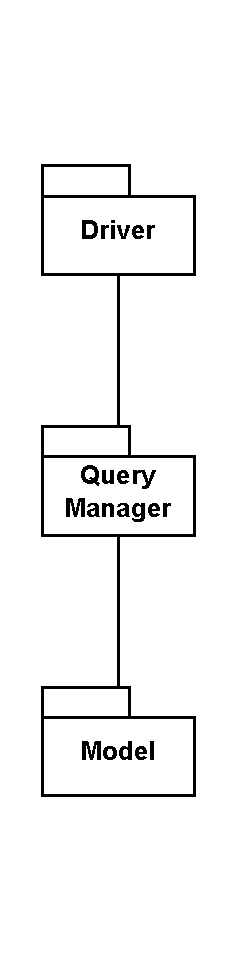
\includegraphics[width=0.2\textwidth]{Images/Integ_0.pdf}
    \caption{Integration Strategy - Step 0}
    \label{fig:integration-strategy-step-0}
\end{figure}

\par The next module that will be implemented and tested will be the Login Manager module, that is the module that will
allow the users to login into the Web Application. 

\begin{figure}[H]
    \centering
    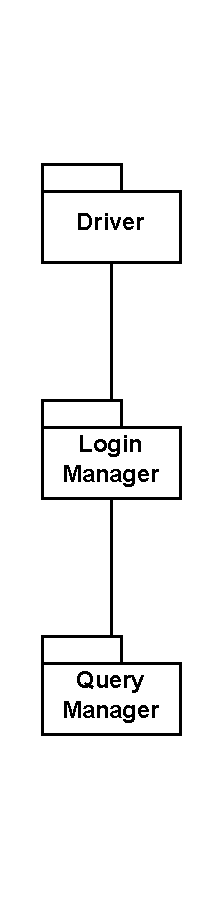
\includegraphics[width=0.2\textwidth]{Images/Integ_1.pdf}
    \caption{Integration Strategy - Step 1}
    \label{fig:integration-strategy-step-1}
\end{figure}

\par the next modules that can be implemented and tested are the Profile Manager module and the Notification Manager. 
Both of these modules are independent of each other and can be implemented and tested simultaneously.
The Notification Manager module is crucial, because a lot of other modules will use it to generate notifications that
will be sent to the users.

\begin{figure}[H]
    \centering
    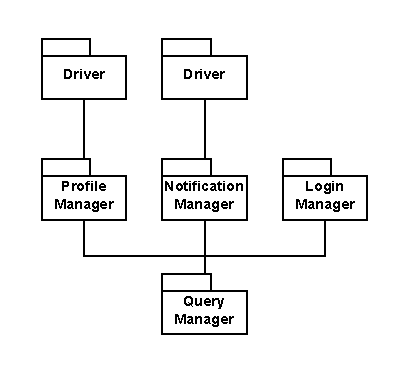
\includegraphics[width=0.5\textwidth]{Images/Integ_2.pdf}
    \caption{Integration Strategy - Step 2}
    \label{fig:integration-strategy-step-2}
\end{figure}

\par The next module that will be implemented and tested will be the Questionnaires Manager module.
For the tidiness of the schemes, from here onward all the modules that will be added will not have the connection to the
Query Manager module in the schema, but only have the connections of the dependencies between the modules.

\begin{figure}[H]
    \centering
    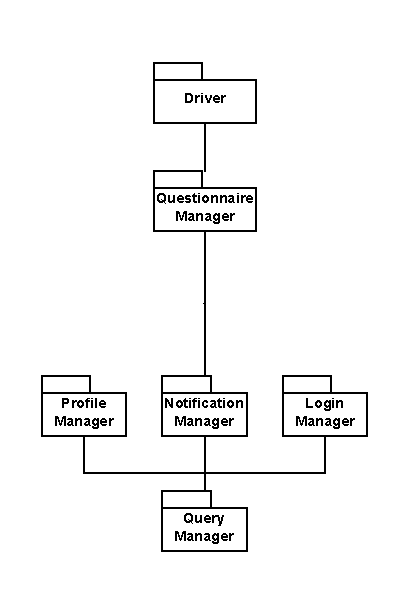
\includegraphics[width=0.5\textwidth]{Images/Integ_3.pdf}
    \caption{Integration Strategy - Step 3}
    \label{fig:integration-strategy-step-3}
\end{figure}

\par The next module that will be implemented and tested will be the Internship Manager module. This module and the previous
one need to be implemented sequentially because the process of creating an internship advertisement will require the 
COs to create a questionnaire that will be sent to the applicants that have applied to the internship.

\begin{figure}[H]
    \centering
    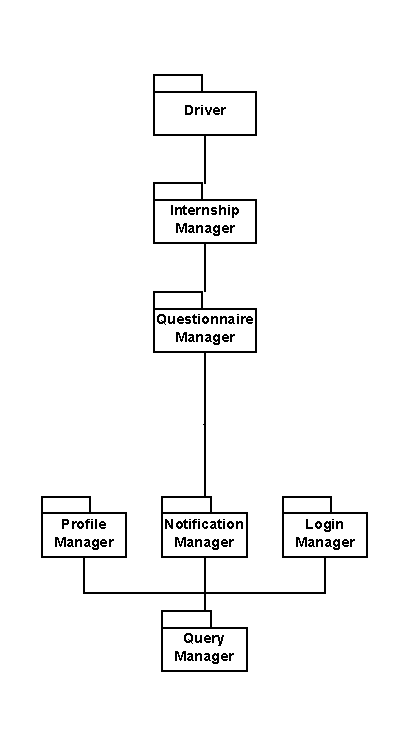
\includegraphics[width=0.5\textwidth]{Images/Integ_4.pdf}
    \caption{Integration Strategy - Step 4}
    \label{fig:integration-strategy-step-4}
\end{figure}

\par The next step of integration will be the implementation and testing of the Complaint Manager module, the Recommendation
Manager module, and the Suggestion Manager module. These modules are independent of each other and can be implemented and
tested simultaneously.

\begin{figure}[H]
    \centering
    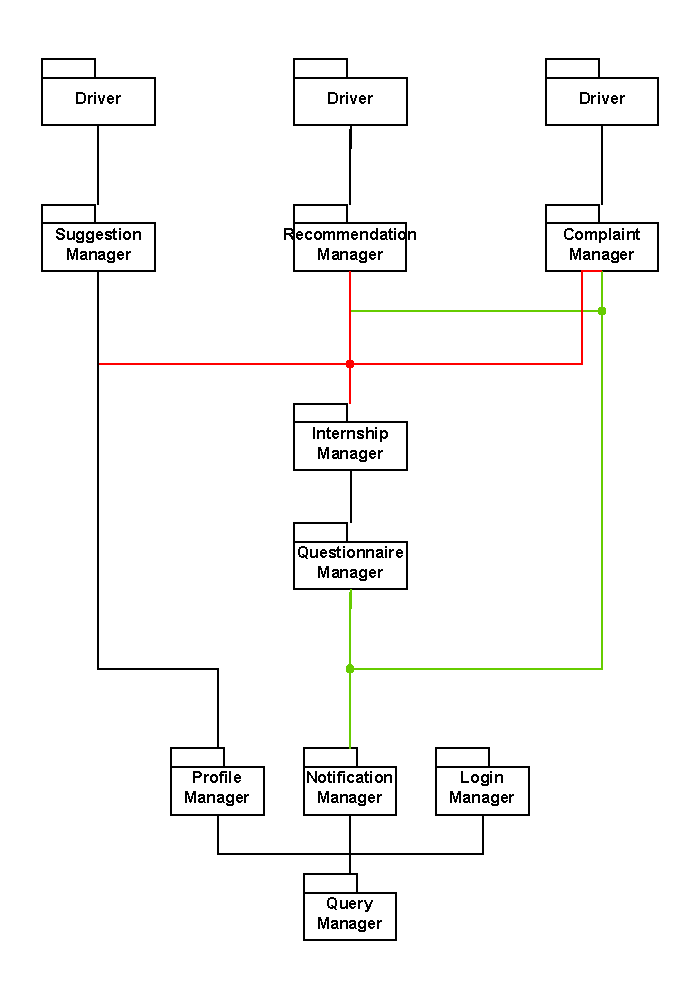
\includegraphics[width=0.5\textwidth]{Images/Integ_5.pdf}
    \caption{Integration Strategy - Step 5}
    \label{fig:integration-strategy-step-5}
\end{figure}

\par The last step of integration will be the implementation and testing of the Dashboard Manager module that requires
all the interfaces of all the other modules except the Query Manager module, to which it doesn't have a direct connection.

\begin{figure}[H]
    \centering
    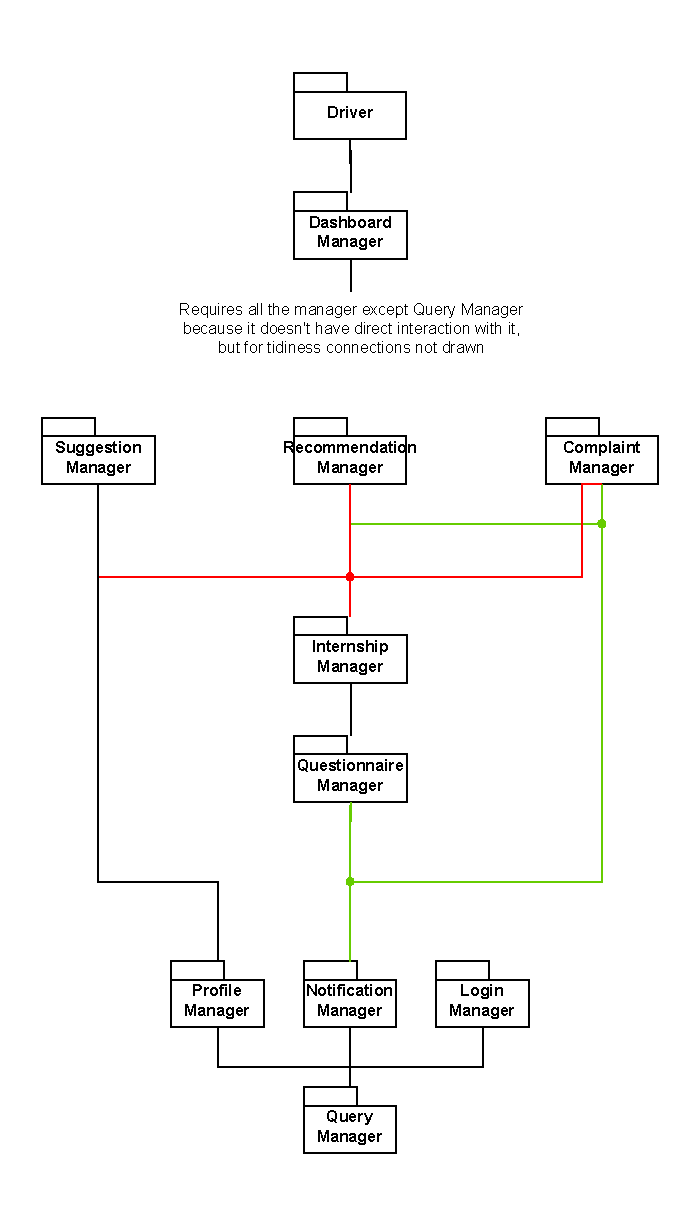
\includegraphics[width=0.5\textwidth]{Images/Integ_6.pdf}
    \caption{Integration Strategy - Step 6}
    \label{fig:integration-strategy-step-6}
\end{figure}

\par The last driver that will be used to test the Dashboard Manager module will simulate the behavior of the Web server
that will simulate the behavior of the Web Application that requires the data that the user needs to see.

\section{System Testing Strategy}

\par After each module is implemented and tested, its time to test the system as a whole. The system testing will be 
done using a Black-Box testing strategy: the system will be tested and evaluated from the user's perspective, without 
any knowledge of the internal architecture.

\par Among all the different types of test that could be conducted, the following are the one that will be detailed and 
conducted:

\begin{enumerate}
    \item \textbf{Functional Testing}: The system will be tested to ensure that all workflows operate as intended and
          meet the specified functional requirements, satisfying user needs.
    \item \textbf{Performance Testing}: The application will undergo tests to confirm it can handle expected user
          loads, sustain peak conditions, and maintain response times within acceptable 
          latency.
    \item \textbf{Security Testing}: The system will be tested to verify that sensitive data is protected, and the
          application is resilient against unauthorized access and common security threats.
    \item \textbf{Failure Testing}: Tests will simulate unexpected scenarios, such as hardware or network failures, to
          confirm that the system can recover gracefully and maintain reliability with 
          minimal disruption.
    \item \textbf{Endurance Testing}: The system will be tested under prolonged usage conditions to ensure stability,
          consistent performance, and the absence of issues like resource exhaustion.
    \item \textbf{User Acceptance Testing}: End-users will validate the application by executing real-world tasks to
          ensure it meets their requirements and is ready for deployment in production environments.
\end{enumerate}
